%ps1.tex
%notes for the course Probability and Statistics COMS10011 
%taught at the University of Bristol
%2019_20 Conor Houghton conor.houghton@bristol.ac.uk

%To the extent possible under law, the author has dedicated all copyright 
%and related and neighboring rights to these notes to the public domain 
%worldwide. These notes are distributed without any warranty. 


\documentclass[11pt,a4paper]{scrartcl}
\typearea{12}
\usepackage{graphicx}
%\usepackage{pstricks}
\usepackage{listings}
\usepackage{color}
\usepackage{tikz}
\usetikzlibrary{decorations.markings}
\lstset{language=C}
\usepackage{fancyhdr}
\pagestyle{fancy}
\lhead{\texttt{cs-uob.github.io/COMS10014/ and github.com/coms10011/2020\_21}}
\lfoot{COMS10014 - P\&C ws1 - Conor}
\begin{document}

\section*{Probability and Combinatorics Worksheet 2}

\subsection*{Useful facts}

\begin{itemize}
\item \textbf{Combinations}: The number of ways of splitting $n$ items into sets of size $r_1$, $r_2$ through to $r_k$ with
  \begin{equation}
    r_1+r_2+\ldots+r_k=n
  \end{equation}
  is
\begin{equation}
\left(\begin{array}{c}n\\r_1,r_2,\ldots,r_k\end{array}\right)=\frac{n!}{r_1!r_2!\ldots r_k!} 
\end{equation}

\item The \textbf{conditional probability} of event $R$ given $C$:
  \begin{equation}
P(R|C)=\frac{P(R\cap C)}{P(C)} 
  \end{equation}
  This is the probability of getting an outcome in event $R$ if we
  know the outcome is in event $C$.

  \end{itemize}

\subsection*{Questions}

These are the questions you should make sure you work on in the workshop.

\begin{enumerate}

\item How many distinct anagrams has the word `BOOKKEEPER'?

\item Two events $A$ and $B$ have probabilities $P(A)=0.2$, $P(B)=0.3$ and $P(A\cup B)=0.4$. Find
\begin{enumerate}
\item Find $P(A\cap B)$.
\item Find $P(\bar{A}\cap \bar{B})$.
\item Find $P(A|B)$.
\end{enumerate}

\item In tic-tac-toe players take turns to write a X or O in a empty location in a $3\times 3$ grid, the grid is traditionally drawn like this
  {\Huge
\begin{center}
\begin{tabular}{c|c|c}
 \phantom{X}&\phantom{O}  &\phantom{O}  \\ \hline
 &\phantom{X}  & \phantom{X}\\ \hline
 &  &\phantom{O}
\end{tabular}
\end{center}
}
  X goes first so after one move the board might look like
  {\Huge
\begin{center}
  \begin{tabular}{c|c|c}
     \phantom{X}&\phantom{O}  &\phantom{O}  \\ \hline
  X&  & \\ \hline
 &  &\phantom{O}
\end{tabular}
\end{center}
}
and if the O player is very poor, or suffering from despair, the game might end after five moves with
  {\Huge
\begin{center}
  \begin{tabular}{c|c|c}
     X&O  &\phantom{O}  \\ \hline
  X&  & \\ \hline
 X&  &O
\end{tabular}
\end{center}
  } A player wins then they have a complete row, column or diagonal,
  in this case X has a column.  How many five move games of
  tic-tac-toe are there?

\item You roll a dice twice, what is the probability the second roll
  has a lower value than the first? You take the ace, two, three,
  four, five and six of hearts to make a mini-pack of cards. You draw
  two cards, what is the probability the second will be lower than the
  first, with the ace counting as a one?

  
\end{enumerate}

\subsection*{Extra questions}

These are questions you can work on in the workshop.

\begin{enumerate}

\item In a lattice path problem you have a two-dimensional lattice
  whose points are located at points with coordinates $(n,m)$ where
  $n$ and $m$ are integers. A lattice path can only have steps that
  increase either the $x$- or $y$-coordinate. This is a $5\times5$ with an example path from (0,0) to (5,5) in red.
\begin{center}
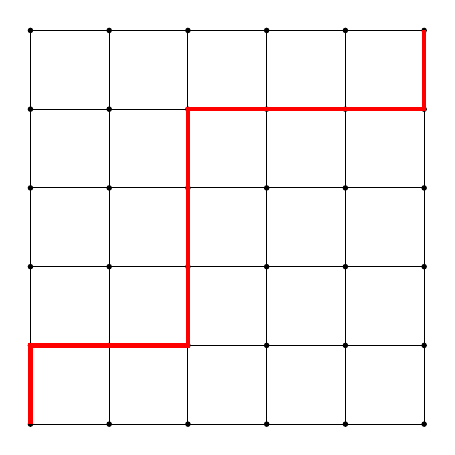
\begin{tikzpicture}
\draw (0,0) grid (5,5);
\foreach \i in {0,...,5}
    \foreach \j in {0,...,5}
    \fill (\i,\j) circle (1pt);
    \draw[ultra thick,red] (0,0) -- (0,1) -- (1,1) -- (2,1) -- (2,2)--(2,3)--(2,4)--(3,4)--(4,4)--(5,4)--(5,5);
\end{tikzpicture}
\end{center}
How many paths are there from (0,0) to (4,5)? If you pick a random path from (0,0) to (4,5) what is the probability it goes through $(2,2)$?

\item How many six move games of tic-tac-toe are there? Remember that
  a six move game can't have been won after five moves.

\item If $p$ is a probability mass function and we define a function on events:
  \begin{equation}
    P(E)=\sum_{x\in E}p(x)
  \end{equation}
  show $P$ is a probability.

\item Ten different objects are put into three boxes. How many different configuations are there? They are sorted so that there are five in the first box, three in the second and two in the third. How many ways configurations are there?
  
\end{enumerate}

\subsection*{Tic-tac-tic-tac-toe}

Tic-tac-toe is a terrible game but tic-tac-tic-tac-toe is
excellent. In tic-tac-tic-tac-toe nine tic-tac-toe boards are arranged
in $3\times 3$ grid so it looks like a big tic-tac-toe board with a
little tic-tac-toe board in each of its nine squares. X can place
their first move in any of the 81 small squares, but from then the
move a player makes determines which small board the other player can
play in; so if X plays the top left square of the small board in the
middle then O must play in the small board in the top left, if they
play the middle square of that small board, then X must play in the
middle small board. When a small board is full, a player directed
there can play in any available square. The winner is the person who
wins the most small games. There is a better description on wikipedia
which calls tic-tac-tic-tac-toe `ultimate tic-tac-toe'.

\end{document}

